\documentclass[10pt,a4paper,twoside]{book}
\usepackage[utf8]{inputenc}
\usepackage[english]{babel}
\usepackage{hyperref}
\usepackage{graphicx}
\graphicspath{{images/}}
%this should make setting iamge maxwidth easier
\makeatletter
\def\maxwidth#1{\ifdim\Gin@nat@width>#1 #1\else\Gin@nat@width\fi}
\makeatother

\usepackage[
    type={CC},
    modifier={by},
    version={4.0},
]{doclicense}

\author{Piotr Halama}
\title{Dragon UnPACKer\\
		User Manual}

\raggedbottom
\begin{document}
\maketitle
\thispagestyle{empty}
\vspace*{\fill}
\noindent
\doclicenseThis
\tableofcontents
\newpage
%\chapter{Word from the book author}

\part{User guide}
\chapter{Installation}
\section{Prerequisites}
\subsection{Operating systems}
This application should run on any Windows from 98 to 10.\\
WINE is supported but it may be slow.
\subsection{Hardware requirements}
If your PC can run Windows it should run this application too.
The lowest tested hardware configuration was PC with 512MB of RAM, Windows 98 SE and graphic card with 32MB of memory.
\newpage

\subsection{Installation process}
\begin{enumerate}
%minipages so items won't break on two pages
\begin{minipage}[t]{\linewidth}
\item Run \textit{setup.exe}\\
\end{minipage}

\begin{minipage}{\linewidth}
\item On newer systems \textbf{User Account Control} window may appear:\\
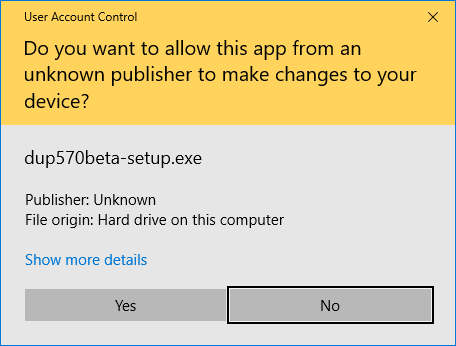
\includegraphics[width=\maxwidth{9cm}]{install/001-uac}\\
Click \textbf{Yes} to allow installation of the Dragon UnPACKer.\\
\end{minipage}

\begin{minipage}[t]{\linewidth}
\item \textbf{Setup} appears.\\
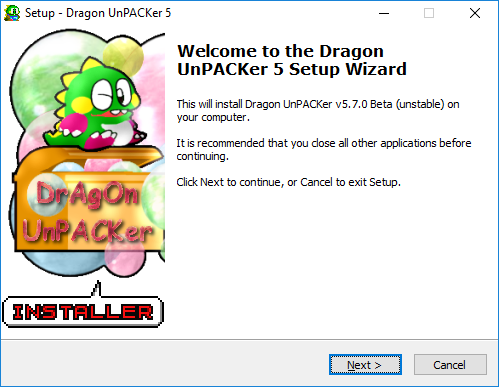
\includegraphics[width=\maxwidth{9cm}]{install/002-start}\\
Click \textbf{Next}.\\
\end{minipage}

\begin{minipage}{\linewidth}
\item \textbf{License Agreement} appears: \\
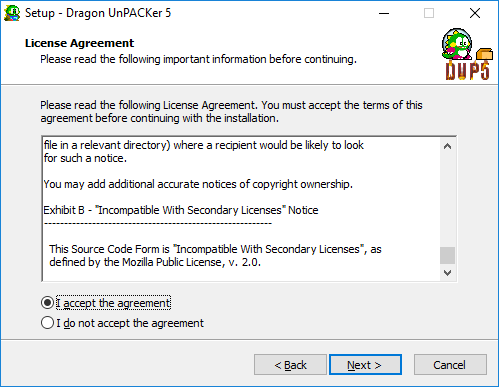
\includegraphics[width=\maxwidth{9cm}]{install/003-license}\\
 Read all the information and click \textbf{I accept the agreement} and \textbf{Next} if you agree with it.\\
\end{minipage}

\begin{minipage}{\linewidth}
\item \textbf{Information} appears: \\
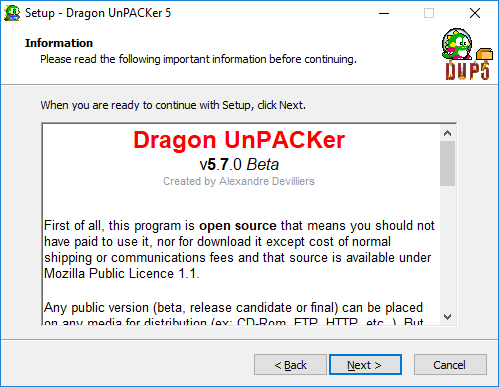
\includegraphics[width=\maxwidth{9cm}]{install/004-information}\\
 Read all the information and click \textbf{Next}.\\
\end{minipage}

\begin{minipage}{\linewidth}
\item \textbf{Select Destination Location} appears:\\
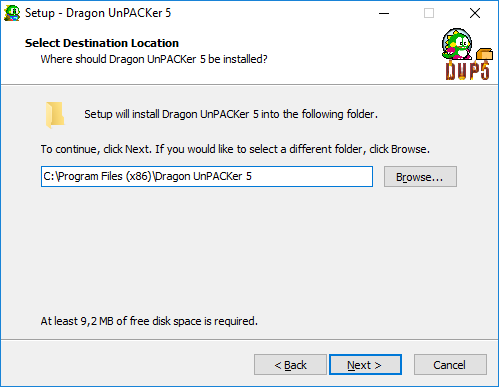
\includegraphics[width=\maxwidth{9cm}]{install/005-destination}\\
You may change installation location by clicking \textbf{Browse} or leave default one, then click \textbf{Next} to continue installing the program.
\end{minipage}

\begin{minipage}{\linewidth}
\item \textbf{Select Start Menu} appears.\\
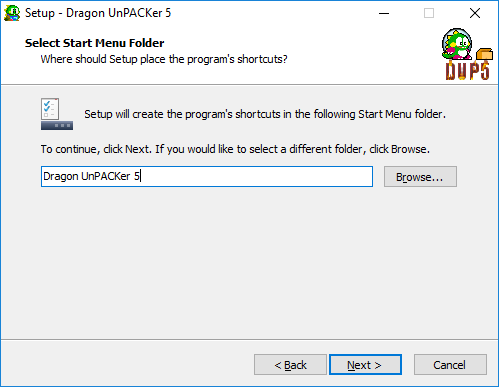
\includegraphics[width=\maxwidth{9cm}]{install/006-menu}\\
You may change start menu folder by clicking \textbf{Browse} or leave default one, then click \textbf{Next} to continue installing the program.
\end{minipage}

\begin{minipage}{\linewidth}
\item \textbf{Select Additional Tasks} appears.\\
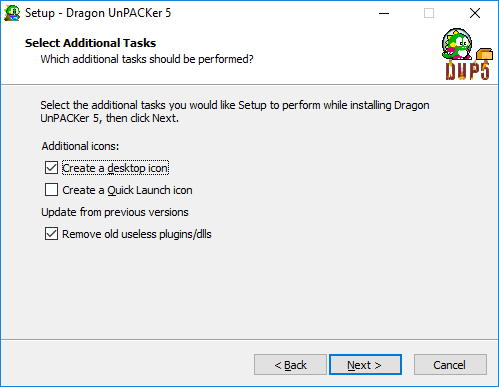
\includegraphics[width=\maxwidth{9cm}]{install/007-additional}\\
Select \textbf{Create a desktop icon} if you want the install program to create an icon for
DragonUnPACKer on your Windows desktop.\\
Select \textbf{Create a Quick Launch icon} if you want the install program to create an icon for
DragonUnPACKer on your Quick Launch bar.\\
Select \textbf{Remove old useless plugins/dlls} if update the install program from previous version to remove old incompatible plugins.\\
When you have selected any options you want, click \textbf{Next}.\\
\end{minipage}

\begin{minipage}{\linewidth}
\item \textbf{Ready to Install} appears.\\
The installation information you have entered so far is summarized.\\
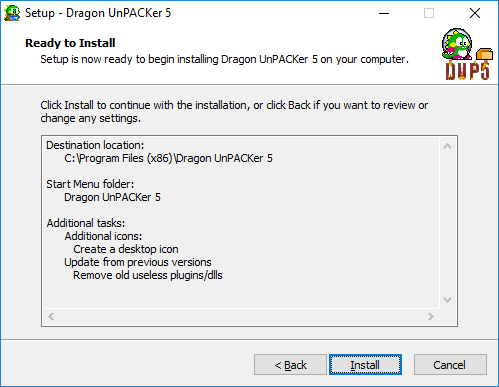
\includegraphics[width=\maxwidth{9cm}]{install/008-summary}\\
If you are satisfied with the summarized information, click \textbf{Next}.\\
If you are not satisfied with the summarized information, click \textbf{Back} until you are at the
installation step where you want to change information. Change the information there, then
click \textbf{Next} until you are back at this screen.\\
\end{minipage}

\begin{minipage}{\linewidth}
\item The installation program begins installing DragonUnPACKer. When the installation is finished, \textbf{Setup} appears.\\
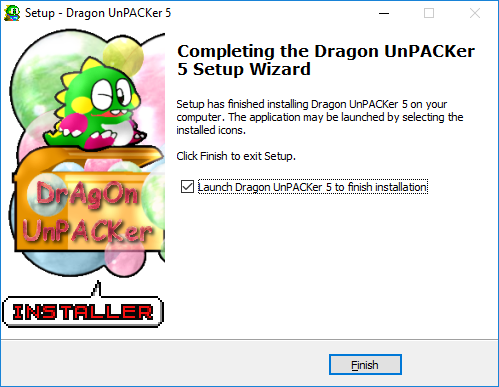
\includegraphics[width=\maxwidth{9cm}]{install/009-finish}\\
Select \textbf{Launch Dragon UnPACKer 5 to finish installation} if you wish to start the program after finishing the installation.\\
When you have selected any options you want, click \textbf{Next}.\\
Click \textbf{Finish}. DragonUnPACKer is now installed on your system.\\
\end{minipage}
\end{enumerate}

%\chapter{Interface}
%\chapter{Duppi}
%\part{Programmer guide}
%\chapter{Driver API}
%\chapter{Translations}
\end{document}